%
% section 6.2.1
%
\subsection{Υπηρεσία Ηλεκτρονικού Ταχυδρομείου E-mail (POP3 - IMAP / SMTP)}

Το ηλεκτρονικό ταχυδρομείο είναι ένα σύστημα για μετάδοση μηνυμάτων μεταξύ υπολογιστών. Στην αρχική του μορφή, το ηλεκτρονικό ταχυδρομείο είχε σχεδιαστεί για να μεταφέρει μηνύματα μόνο κειμένου, αργότερα όμως προστέθηκε η δυνατότητα για μεταφορά εικόνων, ήχου, βίντεο ακόμα και ιστοσελίδων, είτε μέσα στο ίδιο το μήνυμα είτε ως \emph{επισυναπτόμενο αρχείο}. Ο χρήστης e-mail έχει τη δυνατότητα να στέλνει μηνύματα σε άλλους χρήστες της υπηρεσίας άνετα γρήγορα και φθηνά. Το ηλεκτρονικό ταχυδρομείο μπορεί επίσης να στέλνει μηνύματα σε ομάδες χρηστών επιτρέποντας τη δημιουργία \emph{λιστών διανομής ή mailing lists}. Όπως και στο συμβατικό ταχυδρομείο, κάθε χρήστης διαθέτει τη δική του διεύθυνση η οποία είναι γενικά της μορφής:

\begin{center}
xxxxx@yyyyy.zzz
\end{center}

όπου

\begin{itemize}
\item \textbf{xxxxx} είναι το όνομα ή κάποιο ψευδώνυμο του χρήστη
\item \textbf{yyyyy} είναι το όνομα της περιοχής της εταιρίας που παρέχει την υπηρεσία e-mail. Η εταιρία μπορεί να είναι η ίδια που παρέχει υπηρεσίες Internet στον πελάτη ή άλλη εταιρία που παρέχει e-mail επί πληρωμή η δωρεάν. Η περιοχή μπορεί στην πραγματικότητα να περιέχει υποπεριοχές χωρισμένες με τελείες
\item \textbf{zzz} είναι η κατάληξη που αντιστοιχεί στην περιοχή 1ου επιπέδου και συμβολίζει είτε το είδος της εταιρείας που παρέχει την υπηρεσία (.com, .edu, .org κλπ) είτε τη χώρα (.gr, .de, .fr κλπ)
\end{itemize}

Το ηλεκτρονικό ταχυδρομείο είναι μια υπηρεσία που χρησιμοποιεί το μοντέλο πελάτη -- εξυπηρετητή. Πελάτης είναι το πρόγραμμα που χρησιμοποιεί ο χρήστης για να γράψει, να λάβει και να στείλει e-mail (π.χ. Windows Live Mail, Outlook, Mozilla Thunderbird). Ο εξυπηρετητής e-mail (e-mail server) είναι μια δικτυακή υπηρεσία που εκτελείται στον εξυπηρετητή του παροχέα. Σε γενικές γραμμές:

\textbf{Ο Πελάτης (client):}

\begin{itemize}
\item Ξεκινάει την επαφή με τον εξυπηρετητή ταχυδρομείου
\item Ζητά εξυπηρέτηση από τον εξυπηρετητή (π.χ. για να λάβει ή να στείλει mail)
\end{itemize}

\textbf{Ο Εξυπηρετητής (server):}

\begin{itemize}
\item Παρέχει στον πελάτη την εξυπηρέτηση που ζήτησε. Ο εξυπηρετητής είναι υπεύθυνος για να παραδώσει στον πελάτη τα μηνύματα που ήρθαν για αυτόν και να παραδώσει τα μηνύματα που στέλνει ο πελάτης στον εξυπηρετητή προορισμού προκειμένου να παραδοθούν στον πελάτη -- παραλήπτη όταν τα ζητήσει.
\item Κρατά σε ηλεκτρονική θυρίδα (mailbox) τα μηνύματα που δεν έχει ακόμα παραλάβει ο χρήστης. Σε άλλη αντίστοιχη θυρίδα (ουρά) κρατά τα μηνύματα που έχει παραλάβει από το χρήστη μέχρι να μπορέσει να τα αποστείλει στον προορισμό τους.
\end{itemize}

Τα πλεονεκτήματα του ηλεκτρονικού ταχυδρομείου είναι:

\begin{itemize}
\item Είναι πολύ γρήγορο (πρακτικά άμεσο)
\item Ο χρήστης δεν χρειάζεται να παρακολουθεί τη μετάδοση του μηνύματος όπως π.χ. συμβαίνει με το φαξ
\item Είναι πιο οικονομικό από το συμβατικό ταχυδρομείο
\item Μπορούμε να στείλουμε εύκολα το ίδιο μήνυμα σε πολλούς χρήστες ταυτόχρονα
\end{itemize}

Ωστόσο υπάρχουν και μειονεκτήματα:

\begin{itemize}
\item Δεν υπάρχει απόλυτη εγγύηση ότι το μήνυμα έφτασε στο προορισμό του
\item (Εκτός βιβλίου) Λαμβάνουμε μεγάλο αριθμό άσχετων / κακόβουλων μηνυμάτων, ιών κλπ -- γνωστό και ως spam
\end{itemize}

Η μορφή των μηνυμάτων ηλεκτρονικού ταχυδρομείου με μορφή κειμένου καθορίζεται από διεθνές πρότυπο. Ένα τέτοιο μήνυμα αποτελείται από:

\begin{itemize}
\item Την \textbf{επικεφαλίδα (header)}: Είναι ένα σύνολο γραμμών όπου κάθε γραμμή αποτελείται από μια επικεφαλίδα, μια άνω-κάτω τελεία και μια τιμή. Για παράδειγμα:

\begin{verbatim}
From: sonic@thecompany.gr
To: mpampis@othercompany.gr
Subject: Testing Email
\end{verbatim}

\item Το \textbf{σώμα (body)} του μηνύματος: χωρίζεται από την επικεφαλίδα με μια κενή γραμμή. Το σώμα περιέχει το ASCII κείμενο του μηνύματος. Στην πραγματικότητα ακόμα και τα συνημμένα κωδικοποιούνται και μεταδίδονται με αντίστοιχη μορφή. Το τέλος του μηνύματος σηματοδοτείται από μια τελεία ``.'' μόνη της σε μια γραμμή.
\end{itemize}

Τα βασικά πρωτόκολλα που χρησιμοποιούνται για τη διεκπεραίωση των διαδικασιών του ταχυδρομείου είναι τα \textbf{SMTP, POP3, IMAP} και βρίσκονται φυσικά στο επίπεδο εφαρμογής. To SMTP είναι υπεύθυνο για την αποστολή ταχυδρομείου από το πελάτη προς τον εξυπηρετητή και μεταξύ εξυπηρετητών ενώ τα άλλα δύο για τη λήψη μηνυμάτων από τον εξυπηρετητή στον πελάτη.

\begin{inthebox}
\textbf{Με τι μοιάζει μια επικοινωνία SMTP;}

Μπορούμε πράγματι να δούμε και να εκτελέσουμε μια επικοινωνία SMTP στέλνοντας μόνοι μας τις κατάλληλες εντολές, χωρίς να χρειαζόμαστε κάποιο πρόγραμμα ηλεκτρονικού ταχυδρομείου. Γενικά θα πρέπει να θυμάστε ότι στο επίπεδο εφαρμογής οι εντολές των πρωτοκόλλων είναι κατανοητές από τον άνθρωπο: πρόκειται για εντολές στα Αγγλικά, κατά βάση συντομεύσεις (συντμήσεις) λέξεων.

Στο παρακάτω παράδειγμα δείχνουμε πως θα ήταν η επικοινωνία ενός πελάτη με ένα εξυπηρετητή SMTP για την αποστολή ενός μηνύματος. Μπορούμε να εκτελέσουμε χειροκίνητα αυτή τη διαδικασία αν συνδεθούμε με ένα πρόγραμμα ικανό να στείλει ακολουθίες χαρακτήρων (εντολές) στη θύρα 25 (όπου βρίσκεται ο εξυπηρετητής SMTP). Στο παράδειγμα μας χρησιμοποιούμε το πρόγραμμα telnet για να συνδεθούμε σε ένα εξυπηρετητή SMTP που εκτελείται τοπικά σε ένα σύστημα UNIX:

\begin{verbatim}
$ telnet 127.0.0.1 25

Trying 127.0.0.1...
Connected to localhost.
Escape character is '^]'.
220 pegasus.chania-lug.gr ESMTP Sendmail 8.15.2/8.15.2; 
    Thu, 23 Feb 2017 21:28:58 +0200 (EET)
\end{verbatim}

Ο εξυπηρετητής μας απαντάει με το αναγνωριστικό του όπου μπορούμε να δούμε την έκδοση που εκτελεί καθώς και την ημερομηνία ώρα του συστήματος. Για να ξεκινήσουμε την επικοινωνία, στέλνουμε την εντολή ``helo'' ή ``ehlo'' και το όνομα του συστήματος μας για αναγνώριση (και ναι, είναι με ένα ``l'' δεν είναι τυπογραφικό!)

\begin{verbatim}
helo localhost
250 pegasus.chania-lug.gr Hello localhost [127.0.0.1],
    pleased to meet you
\end{verbatim}

Ο εξυπηρετητής μας απαντάει με ένα μήνυμα καλωσορίσματος. Τώρα πρέπει να προχωρήσουμε στέλνοντας τα στοιχεία της επικεφαλίδας, και ακολούθως τα δεδομένα. Ξεκινάμε με την επικεφαλίδα:

\begin{verbatim}
mail from: sonic@chania-lug.gr
250 2.1.0 sonic@chania-lug.gr... Sender ok
\end{verbatim}

Ο εξυπηρετητής επιβεβαιώνει ότι η διεύθυνση αποστολέα είναι δεκτή.

\begin{verbatim}
rcpt to: mpampis@freebsdworld.gr
250 2.1.5 mpampis@freebsdworld.gr... Recipient ok
\end{verbatim}

Επιβεβαιώνεται επίσης η διεύθυνση παραλήπτη. Είμαστε έτοιμοι να στείλουμε το σώμα του email γράφοντας την εντολή ``data'' (στο παράδειγμα μας παραλείψαμε το θέμα):

\begin{verbatim}
data
354 Enter mail, end with "." on a line by itself
\end{verbatim}

Ο εξυπηρετητής μας προτρέπει να γράψουμε το μήνυμα μας και να τελειώσουμε με μια τελεία ``.'' σε μια γραμμή από μόνη της.

\begin{verbatim}
Hello, this is a test mail
.
250 2.0.0 v1NJaK3Q095307 Message accepted for delivery
\end{verbatim}

Ο εξυπηρετητής επιβεβαιώνει ότι δέχτηκε να παραδώσει το μήνυμα μας στον παραλήπτη. Σε αυτό το σημείο, μπορούμε να αποσυνδεθούμε από τον εξυπηρετητή.

\begin{verbatim}
quit
221 2.0.0 pegasus.chania-lug.gr closing connection
\end{verbatim}


Στην πραγματικότητα κάθε φορά που στέλνετε ένα mail μέσω ενός προγράμματος όπως το Thunderbird, το πρόγραμμα στέλνει αυτές τις εντολές για εσας. Όπως βλέπετε δεν υπάρχει κάτι το μυστηριώδες στις εντολές πρωτοκόλλων του επιπέδου εφαρμογής!\\
\end{inthebox}

\textbf{Πως ολοκληρώνεται η προηγούμενη επικοινωνία;} Ο εξυπηρετητής που παρέλαβε το μήνυμα μας θα βρει (μέσω ερωτήματος στο DNS) ποιος είναι ο εξυπηρετητής ταχυδρομείου που είναι υπεύθυνος για την περιοχή που ανήκει ο παραλήπτης (στο παράδειγμα, θα ψάξει ποιος εξυπηρετητής ταχυδρομείου είναι υπεύθυνος για τον τομέα freebsdworld.gr π.χ. ο mail.freebsdworld.gr). Έπειτα θα επικοινωνήσει με τον εξυπηρετητή αυτό χρησιμοποιώντας πάλι το πρωτόκολλο SMTP και θα του παραδώσει το μήνυμα για το χρήστη mpampis. Ο παραλήπτης του μηνύματος θα συνδεθεί με το δικό του πρόγραμμα (π.χ. Thunderbird, σχήμα \ref{6-7}) και θα κατεβάσει το μήνυμα από το διακομιστή χρησιμοποιώντας το πρωτόκολλο POP3 ή IMAP.


\begin{itemize}
\item Το πρωτόκολλο \textbf{SMTP, Simple Mail Transfer Protocol} ή Πρωτόκολλο Μεταφοράς Απλών Μηνυμάτων χρησιμοποιείται όταν παραδίδεται ένα μήνυμα από ένα πελάτη προς ένα διακομιστή ηλεκτρονικού ταχυδρομείου προκειμένου να παραδοθεί σε ένα παραλήπτη. Χρησιμοποιείται επίσης και για την αποστολή μηνυμάτων μεταξύ εξυπηρετητών e-mail. Το SMTP παραδοσιακά χρησιμοποιεί τη θύρα 25 όπου τα μηνύματα μεταδίδονται χωρίς κρυπτογράφηση, ενώ οι σύχρονες εκδοχές χρησιμοποιούν τη θύρα 465 για κρυπτογραφημένη επικοινωνία SSL ή την 587 για TLS.
\item Το πρωτόκολλο \textbf{POP3, Post Office Protocol 3} ή πρωτόκολλο ταχυδρομικού γραφείου χρησιμοποιείται στο πρόγραμμα -- πελάτη (e-mail client) προκειμένου να συνδεθεί στον διακομιστή ταχυδρομείου και να κατεβάσει τα μηνύματα ηλεκτρονικού ταχυδρομείου στον τοπικό υπολογιστή. Το πρωτόκολλο αυτό είναι αρκετά απλό και δεν προσφέρει ιδιαίτερες δυνατότητες εκτός από τη λήψη. Μετά τη σύνδεση και την επαλήθευση στοιχείων κατεβάζει όλα τα μηνύματα από τον εξυπηρετητή στο τοπικό μηχάνημα και κατόπιν τα διαγράφει από τον εξυπηρετητή και αποσυνδέεται. Υπάρχει η δυνατότητα να παραμείνουν αντίγραφα των μηνυμάτων στο διακομιστή μέσω ρύθμισης στο e-mail client. Το POP3 χρησιμοποιεί τη θύρα 110 ενώ η παραλλαγή με κρυπτογράφηση χρησιμοποιεί την 995 (SSL).
\item Το πρωτόκολλο \textbf{IMAP, Internet Message Access Protocol} ή πρωτόκολλο πρόσβασης ηλεκτρονικού ταχυδρομείου έχει αρκετά παρόμοια χαρακτηριστικά με το POP3 αλλά και πρόσθετες δυνατότητες. Πρόκειται επίσης για πρωτόκολλο που χρησιμοποιείται για να κατεβάσει ο πελάτης τα μηνύματα από ένα διακομιστή ταχυδρομείου. Έχει σχεδιαστεί για να επιτρέπει στους χρήστες να διατηρούν τα mail τους στον διακομιστή αντί να τα κατεβάζουν εξ'ολοκλήρου στον τοπικό τους υπολογιστή. Το IMAP απαιτεί περισσότερο χώρο στο δίσκο του κεντρικού υπολογιστή ταχυδρομείου (mail server) και περισσότερη υπολογιστική ισχύ (CPU) από το POP3 καθώς τα μηνύματα παραμένουν στο διακομιστή. Το IMAP χρησιμοποιεί τη θύρα TCP 143 ή την 993 για κρυπτογραφημένη επικοινωνία (SSL).
\end{itemize}

\begin{figure}[!ht]
 \centering
 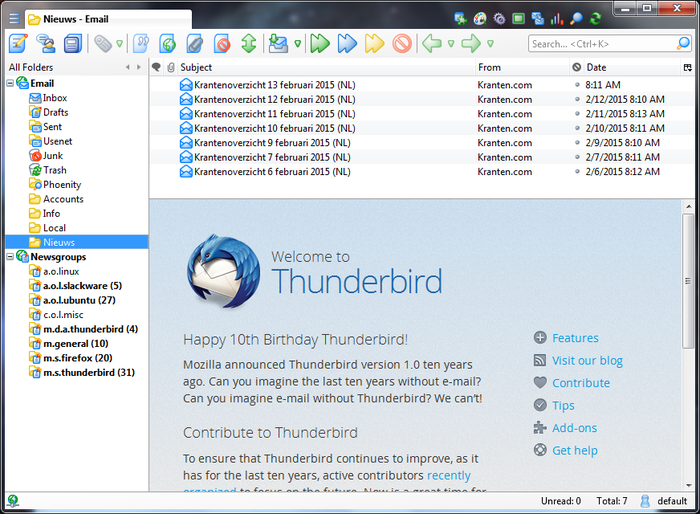
\includegraphics[width=0.95\textwidth]{images/chapter6/6-7}
 \caption {\textsl{To Πρόγραμμα Thunderbird (e-mail client)}}
 \label{6-7}
\end{figure}

Ένας διαφορετικός τύπος ηλεκτρονικού ταχυδρομείου είναι το \emph{Web mail} που χρησιμοποιεί το πρωτόκολλο HTTP για να ολοκληρωθεί η επικοινωνία διαβάζεται μέσα από κάποιο browser (φυλλομετρητή). Αυτό το είδος ηλεκτρονικού ταχυδρομείου είναι μια υπηρεσία του Παγκόσμιου Ιστού (World Wide Web). 

Για να μπορέσει ένας χρήστης να διαβάσει τα μηνύματα του, θα πρέπει να πιστοποιηθεί από τον εξυπηρετητή εισερχόμενης αλληλογραφίας (POP3 ή IMAP) χρησιμοποιώντας κατάλληλο όνομα χρήστη (User Id ή Login) και κωδικό (Password). Ετσί μπορεί να διαπιστωθεί ότι είναι πράγματι ο χρήστης στον οποίο αντιστοιχεί η ηλεκτρονική διεύθυνση που προσπαθεί να προσπελάσει.